% Asset ID: A22FurtherKinematicsTikZ-006
% Unit: A22
% Topic: Further Kinematics
% Related section: Method decision flow
\documentclass[tikz,border=8pt]{standalone}
\usepackage{amsmath}
\usetikzlibrary{arrows.meta,positioning,angles,quotes}
\begin{document}

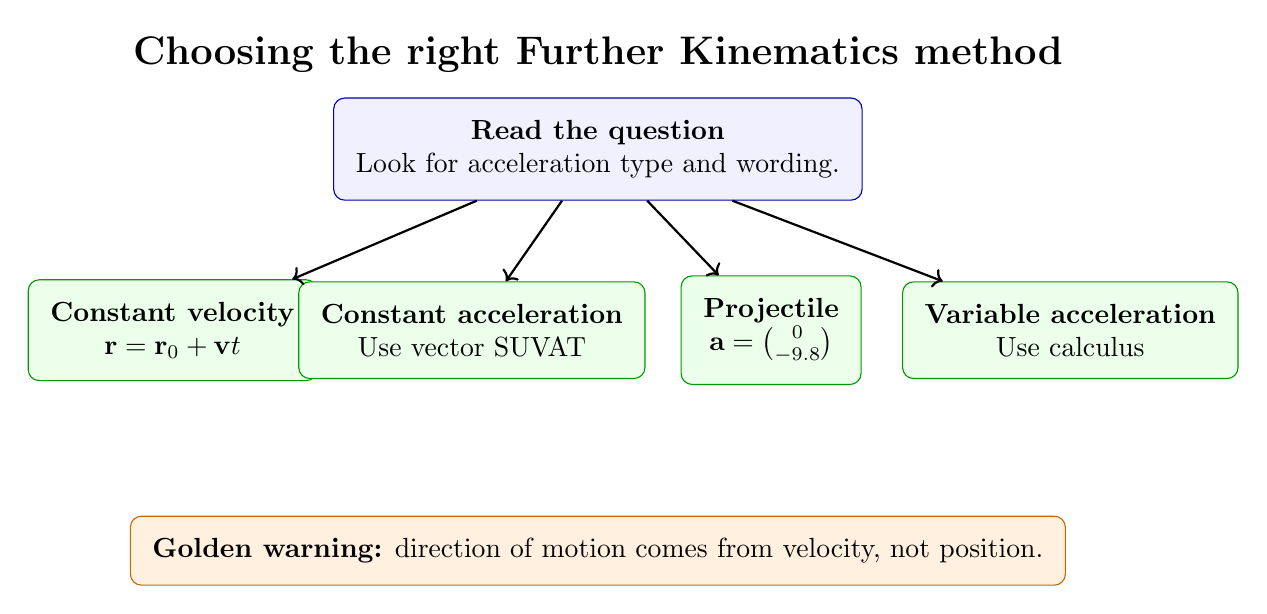
\begin{tikzpicture}[start/.style={draw=blue!70!black,fill=blue!6,rounded corners,align=center,inner sep=8pt}, method/.style={draw=green!60!black,fill=green!8,rounded corners,align=center,inner sep=8pt}, output/.style={draw=orange!80!black,fill=orange!12,rounded corners,align=center,inner sep=8pt}, arrow/.style={->,thick}]
\node[font=\bfseries\Large] at (7,8) {Choosing the right Further Kinematics method};
\node[start] (read) at (7,6.8) {\textbf{Read the question}\\Look for acceleration type and wording.};
\node[method] (cv) at (1.6,4.5) {\textbf{Constant velocity}\\$\mathbf r=\mathbf r_0+\mathbf vt$};
\node[method] (ca) at (5.4,4.5) {\textbf{Constant acceleration}\\Use vector SUVAT};
\node[method] (proj) at (9.2,4.5) {\textbf{Projectile}\\$\mathbf a=\binom{0}{-9.8}$};
\node[method] (var) at (13,4.5) {\textbf{Variable acceleration}\\Use calculus};
\draw[arrow] (read)--(cv); \draw[arrow] (read)--(ca); \draw[arrow] (read)--(proj); \draw[arrow] (read)--(var);
\node[output] at (7,1.7) {\textbf{Golden warning:} direction of motion comes from velocity, not position.};
\end{tikzpicture}
\end{document}
